% Drawing 142/06-6 -- folder 142, batch 06, archive page 107 (PDF page 108).
% Transcription: Au crayon, deux sphères. La première : pôles $0$ (en haut) et $\infty$ (en bas), méridiens et équateur ; sur l'équateur, quatre petits cercles orientés autour de $1$, $i$, $-1$, $-i$ (étiquettes partiellement lisibles), reliés aux pôles par des chemins fléchés, certains en pointillé.
% Kind: sphere with poles, meridians and small oriented circles. Method 2 (schematic redraw from the facsimile). Status: partial.
% Notes: In pencil: outline, the pole circles 0 (top) and infinity (bottom), the equator (back half dashed), four small oriented circles on the equator; arrowed paths from the top pole down to the circles (two seen, solid; two hidden, dashed) and thin meridians down to the bottom pole. Labels: "1" at the left circle and "i" at the front one are legible; the right one reads like "-1"; the back circle is unlabelled (-i by elimination). The formula "1 -> F_2^2" on the right is text, not drawn.
% Coordinates: 1 unit = 1 mm = 1/100 of the crop width (bbox in page fractions: [0.1, 0.08, 0.58, 0.43]).
% Redrawn by Claude (claude-opus-5-5), issue #73, 2026-11-07; not checked by a human; not compiled (no TeX in the session).
% Rights: reproduces part of the work -- behind RENDER_TRANSCRIPTS, never published by itself.
\documentclass[tikz,border=3pt]{standalone}
\usepackage{amsmath,amssymb}
\usetikzlibrary{patterns,arrows.meta}
\tikzset{pencil/.style={black!45}, struck/.style={black!35}, mark/.style={circle,draw,inner sep=1.3pt}, pt/.style={circle,fill,inner sep=0.9pt}, opt/.style={circle,draw,fill=white,inner sep=1.1pt}}
\begin{document}
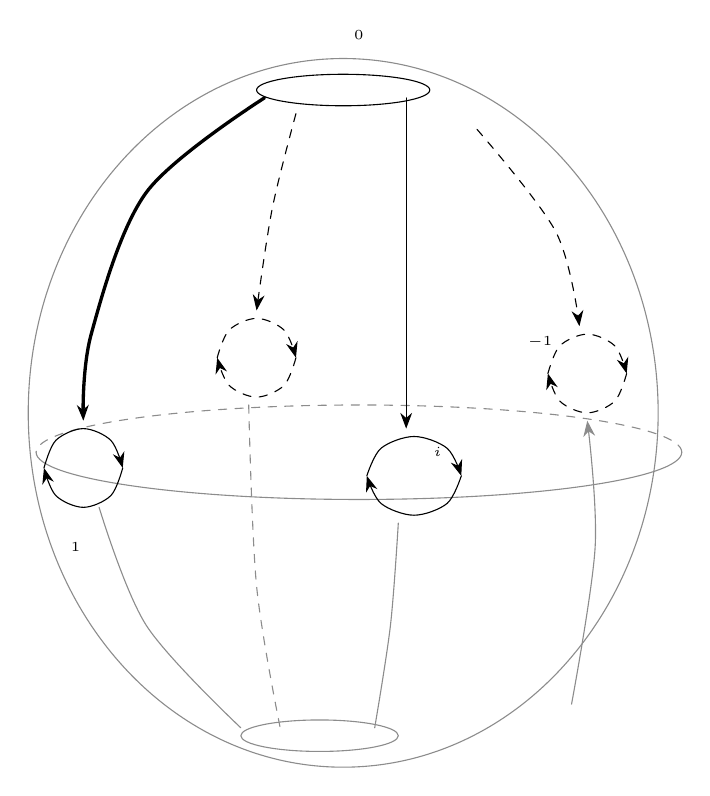
\begin{tikzpicture}[x=1mm,y=1mm,line cap=round,line join=round,font=\scriptsize]
\draw[pencil] (53,-58) ellipse[x radius=40, y radius=45];
\draw (53,-17) ellipse[x radius=11, y radius=2];
\draw[pencil] (50,-99) ellipse[x radius=10, y radius=2];
\node[inner sep=1pt] at (55,-10) {\tiny $0$};
\draw[pencil] (14,-63) arc[start angle=180, end angle=360, x radius=41, y radius=6];
\draw[pencil,dashed] (96,-63) arc[start angle=0, end angle=180, x radius=41, y radius=6];
\draw[-{Stealth[length=2mm]}] plot[smooth, tension=0.55] coordinates {(15,-65) (16.5,-61.5) (20,-60) (23.5,-61.5) (25,-65)};
\draw[-{Stealth[length=2mm]}] plot[smooth, tension=0.55] coordinates {(25,-65) (23.5,-68.5) (20,-70) (16.5,-68.5) (15,-65)};
\draw[-{Stealth[length=2mm]},dashed] plot[smooth, tension=0.55] coordinates {(37,-51) (38.5,-47.5) (42,-46) (45.5,-47.5) (47,-51)};
\draw[-{Stealth[length=2mm]},dashed] plot[smooth, tension=0.55] coordinates {(47,-51) (45.5,-54.5) (42,-56) (38.5,-54.5) (37,-51)};
\draw[-{Stealth[length=2mm]}] plot[smooth, tension=0.55] coordinates {(56,-66) (57.8,-62.5) (62,-61) (66.2,-62.5) (68,-66)};
\draw[-{Stealth[length=2mm]}] plot[smooth, tension=0.55] coordinates {(68,-66) (66.2,-69.5) (62,-71) (57.8,-69.5) (56,-66)};
\draw[-{Stealth[length=2mm]},dashed] plot[smooth, tension=0.55] coordinates {(79,-53) (80.5,-49.5) (84,-48) (87.5,-49.5) (89,-53)};
\draw[-{Stealth[length=2mm]},dashed] plot[smooth, tension=0.55] coordinates {(89,-53) (87.5,-56.5) (84,-58) (80.5,-56.5) (79,-53)};
\draw[-{Stealth[length=2mm]},very thick] plot[smooth, tension=0.55] coordinates {(43,-18) (28,-30) (21,-48) (20,-59)};
\draw[-{Stealth[length=2mm]}] (61,-18) -- (61,-60);
\draw[dashed,-{Stealth[length=2mm]}] plot[smooth, tension=0.55] coordinates {(47,-20) (44,-32) (42,-45)};
\draw[dashed,-{Stealth[length=2mm]}] plot[smooth, tension=0.55] coordinates {(70,-22) (80,-35) (83,-47)};
\draw[pencil] plot[smooth, tension=0.55] coordinates {(22,-70) (28,-85) (40,-98)};
\draw[pencil] plot[smooth, tension=0.55] coordinates {(60,-72) (59,-85) (57,-98)};
\draw[pencil,dashed] plot[smooth, tension=0.55] coordinates {(41,-57) (42,-80) (45,-98)};
\draw[pencil,-{Stealth[length=2mm]}] plot[smooth, tension=0.55] coordinates {(82,-95) (85,-75) (84,-59)};
\node[inner sep=1pt] at (19,-75) {\tiny $1$};
\node[inner sep=1pt] at (65,-63) {\tiny $i$};
\node[inner sep=1pt] at (78,-49) {\tiny $-1$};
\end{tikzpicture}
\end{document}
